\documentclass[11pt]{article}

\usepackage{imports}

%%%%%%
%Ornament Pacakages
\usepackage[object=vectorian]{pgfornament}
\usepackage{lmodern}   
\usepackage[utf8]{inputenc} 
\usepackage[T1]{fontenc} 
\usepackage{adforn}
\usepackage{lmodern}
\pdfmapfile{+ OrnementsADF.map}
\usepackage{adforn}
%%%%%%%

\usepackage{tikz}
\usetikzlibrary{arrows}
\usetikzlibrary{calc}
\usepackage{tikzrput}

\usepackage{semantic}

\usetikzlibrary{calc,trees,positioning,arrows,chains,shapes.geometric,%
    decorations.pathreplacing,decorations.pathmorphing,shapes,%
    matrix,shapes.symbols}
    
    \usetikzlibrary{positioning}

\usetikzlibrary{shapes.multipart}

\usepackage{listings}
\usepackage{synttree}

\usepackage{nicefrac}
\usepackage{diagbox}

\usepackage{setspace}
\usepackage{anysize}
\usepackage{CJKutf8}


\usepackage{fancyhdr}
\pagestyle{fancy}
\fancyhead[L]{\adforn{34} \textit{Snippet Compilation}}
\fancyhead[R]{Bryce Evanas}

\fancyfoot[C]{$\quad  \quad \quad \quad \quad \quad \quad \, \, \, \, \,$ --~\thepage~--}

%block style
\setlength\parindent{0pt}

\setlength{\topmargin}{-.5in}
\setlength{\textheight}{9in}
\setlength{\oddsidemargin}{.125in}
\setlength{\textwidth}{6.25in}

\begin{document}

\title{\LaTeX\, Snippet Compilation}
\maketitle


\tikzstyle{label} = [ -latex',draw=none, fill=none, minimum height=2em]

\section{TikZ Graphs}

\subsection*{Clique}
\begin{center}

\begin{tikzpicture}
[>=stealth',scale=.2,auto=center,every node/.style={circle,fill=blue!10,minimum size=3em,draw}]

\node[fill=purple!20] (a) at (21.8,-8.6) {};
\node[fill=purple!20] (b) at (38,-16) {};
\node[fill=purple!20] (c) at (35.5,-31.1) {};
\node[fill=purple!20] (d) at (18.8,-34.5) {};
\node[fill=purple!20] (e) at (11,-20.3) {};

\node (f) at (53.3,-23.9) {};
\node (g) at (49.9,-37.5) {};
\node (h) at (26.1,-42.9) {};
\node (i) at (38.8,-45.3) {};
\node (j) at ((12.3,-44.3) {};

\node[fill=green!20] (v1) at (-5,-10) {$v_1$};
\node[fill=green!20] (v2) at (-5,-24) {$v_2$};

%clique
\foreach \from/\to in {a/b,a/c,a/d,a/e,b/c,b/d,b/e,c/d,c/e,d/e}
\draw (\from) edge(\to);

\foreach \from/\to in {b/f,c/f,c/g,i/h,d/h,c/i,d/j}
\draw (\from) edge(\to);

\foreach \to in {a,b,c,d,e,f,g,h,i,j}
\draw [green] (v1) edge [dashed] (\to);

\foreach \to in {a,b,c,d,e,f,g,h,i,j}
\draw [green] (v2) edge [dashed] (\to);

\end{tikzpicture}\\
Graph $G$ with clique $k_5$ highlighted in red and $v_1,v_2$ connected to every vertex in $G$. A near clique of size $k+2$ forms between the red and green colored nodes.
\end{center}

\tikzset{
>=stealth',
  punktchain/.style={
    rectangle, 
    rounded corners, 
    % fill=black!10,
    draw=black, very thick,
    text width=8em, 
    minimum height=2.5em, 
    text centered, 
    on chain},
  line/.style={draw, thick, <-},
  element/.style={
    tape,
    top color=white,
    bottom color=blue!50!black!60!,
    minimum width=8em,
    draw=blue!40!black!90, very thick,
    text width=10em, 
    minimum height=3.5em, 
    text centered, 
    on chain},
  every join/.style={->, thick,shorten >=1pt},
  decoration={brace},
  tuborg/.style={decorate},
  tubnode/.style={midway, right=2pt},
   arr/.style={join,thick,->,shorten >=1pt},
}

\begin{minipage}{\textwidth}


\textbf{Flow chart style graph}
\begin{center}
\begin{tikzpicture}
  [ start chain=going]
  \definecolor{coolblu}{rgb}{0,0.6,0.6};
  % HACK... no idea why the 2.69... random number making it work
     \node[punktchain, draw = coolblu] (a) at (2.69,10) {\texttt{i := 0}};
     \node[punktchain, draw = coolblu] (if) at (0,8)      {\texttt{while i < 10}};
     \node[punktchain, draw = coolblu] (inc)  at (3,6) {\texttt{i := i + 1}};
     \node[punktchain, draw = coolblu] (cont)  at (0,4) {$\vdots$};

     \draw[arr] (2.69,11.5) to node[label, left]  {$\bot$} (a);
     \draw[arr] (a) to node[label, left]  {$[0,0]$} (if);
     
     
       \draw[arr,bend left] (if) to node[label, right]  {$[0,9]$} (inc);
       \draw[arr,bend left] (inc) to node[label, right]  {$[1,10]$} (if);
       
       
        \draw[arr] (if) to node[label, left]  {$[10,10]$} (cont);
      \draw[arr] (cont) to (2.69,2.5);

  \end{tikzpicture}
\end{center}
\end{minipage}
\vspace{8mm}
\textbf{Bipartite Graphs}
 \begin{center}
\begin{tikzpicture}
[>=stealth',scale=1,auto=center,every node/.style={circle,fill=blue!10,minimum size=3em,draw}]


\node (l1) at (4,6) {};
\node (l2) at (4,4) {};
\node (l3) at (4,2) {};

\node[fill=green!20] (r1) at (0,6) {};
\node[fill=green!20] (r2) at (0,4) {};
\node[fill=green!20] (r3) at (0,2) {};


\draw (l1) edge[dashed]  (r1);
\draw (l1) edge  (r2);
\draw (l1) edge[dotted]  (r3);

\draw (l2) edge[dashed]  (r2);
\draw (l2) edge  (r3);
\draw (l2) edge[dotted]  (r1);


\draw (l3) edge[dashed]  (r3);
\draw (l3) edge  (r1);
\draw (l3) edge[dotted]  (r2);

\end{tikzpicture}
\end{center}

\textbf{Doubly labeled nodes, Flow Graph}
\begin{center}
\begin{tikzpicture}[>=stealth',scale=1,auto=center,every node/.style={circle,fill=blue!10,minimum size=2.5em,draw}]
\tikzstyle{label} = [ -latex',draw=none, fill=none, minimum height=2em]
\node[label] (sl) at (0,.7) {$\Phi(s)$};
\node (s) at (0,0) {$\phi_0$};

\node[label] (il) at (5,1.7) {$\Phi(s'_i,s_{-i})$};
\node (i) at (5,1) {$\phi_i$};

\node[label] (jl) at (5,-.3) {$\Phi(s'_j,s_{-j})$};
\node (j) at (5,-1) {$\phi_j$};

\node[label] (ijl) at (10,.7) {$\Phi(s'_{ij},s_{-i-j})$};
\node (ij) at (10,0) {$\phi_{ij}$};


\draw[->] (s) edge (i);
\draw[->] (s) edge (j);
\draw[->] (i) edge (ij);
\draw[->] (j) edge (ij);
\end{tikzpicture}
\end{center}
\textbf{Side by side graphs, bended labeled edges}
\begin{center}
\begin{multicols}{2}
\begin{minipage}[5cm]{\textwidth/2}
\vspace{10.5mm}
\begin{tikzpicture}[>=stealth',scale=.5,auto=center,every node/.style={circle,fill=blue!10,minimum size=3em,draw}]

\node (a) at (0,0) {};
\node (b) at (10,0) {};
\draw[->] (a) edge[bend right] (b) ;
\draw[->] (a) edge[bend left] (b) ;
\end{tikzpicture}
\end{minipage}
\begin{minipage}[5cm]{\textwidth/2}
\begin{tikzpicture}[>=stealth',scale=.5,auto=center,every node/.style={circle,fill=blue!10,minimum size=3em,draw}]

\node (a) at (0,0) {};
\node (b) at (10,0) {};
\draw[->,bend left] (a) to node[minimum size=1em,label, above]  {$c_e(x)$} (b);
\draw[->,bend right] (a) to node[minimum size=1em,label,below]  {$c_e'(x)$} (b);
\end{tikzpicture}
\end{minipage}
\end{multicols}
\end{center}

\textbf{Anotated Graph}

\begin{center}
\begin{minipage}{\textwidth*3/7}
$$
c_e(s) =
\begin{cases}
-u_i(s), & x_e = n \\
0, & \text{otherwise}
\end{cases}$$
\vspace{5mm}
$$
c_e'(s) =
\begin{cases}
-c_e(s), & x_e = n-1 \\
0, & \text{otherwise}
\end{cases}
$$
\end{minipage}
\begin{minipage}{\textwidth*3/7}
\begin{tikzpicture}
[>=stealth',scale=3,auto=center,every node/.style={circle,fill=blue!10,minimum size=3.5em,draw}]

\node[fill=red!20] (a) at (1,1) {$2$};
\node[fill=red!20,minimum size=1em] at (0.5,1) {};
\node (b) at (1,2) {$1$};
\node[minimum size=1em]  at (0.5,2) {};
\node[label] (a) at (1,2.5) {Player $A$'s Set};

\node (c) at (2,1) {$1$};
\node[minimum size=1em]  at (2.5,1) {};
\node[fill=red!20] (d) at (2,2) {$2$};
\node[fill=red!20,minimum size=1em]  at (2.5,2) {};
\node[label] (a) at (2,2.5) {Player $B$'s Set};


\draw[orange!70,ultra thick,dotted] (.7,.7)  rectangle (1.3,2.3);
\draw[purple!70,ultra thick,dotted] (1.7,.7)  rectangle (2.3,2.3);
\end{tikzpicture}
\end{minipage}
\end{center}



\begin{center}
\adforn{21}\quad\adforn{11}\quad\adforn{49}\\
\end{center}


\subsection*{Subgraph}
\begin{center}
\begin{tikzpicture}
[>=stealth',scale=1.2,auto=center,every node/.style={circle,fill=blue!10,minimum size=3.5em,draw}]

\node (a) at (.5,.5) {1};
\node[fill=purple!20] (b) at (2,2) {2};
\node[fill=purple!20] (c) at (2.2,4) {3};
\node[fill=purple!20] (d) at (4,3) {4};
\node (e) at (6,3.5) {5};
\node (f) at (6,2) {6};
\node (g) at (7.7,4) {7};


\foreach \from/\to in {a/b,b/c,b/d,c/d,d/e,e/g,e/f}
\draw (\from) edge(\to);

\draw[red,thick,dotted] (1,4.75)  rectangle (4.75,1.25);

\end{tikzpicture}\\
Graph $G$ with clique $k_3$ highlighted.
\end{center}

\textbf{Runtime of $\sigma$}
\begin{align*}
&\text{Add nodes $v_1,v_2$: } &O(1)\\ 
&\text{Connect $v_1,v_2$ to $v\, \forall v \in V$: } &O(V)\\ 
&\textbf{Total Reduction Runtime: } &O(V)\\
\end{align*}

\section{Matrices}
 
\[M_k = 
\left[ {\begin{array}{*{3}c}
   2 & 1 & 1  \\
   1 & 2 & 1 \\
   1 & 1 & 2  \\
 \end{array} } \right]
\quad
 M_G = 
\left[ {\begin{array}{*{7}c}
   2 & 1 & 0 & 0 & 0 & 0 & 0  \\
   1 & \textcolor{red}2 & \textcolor{red}1 & \textcolor{red}1 & 0 & 0 & 0  \\
   0 & \textcolor{red}1 & \textcolor{red}2 & \textcolor{red}1 & 0 & 0 & 0  \\
   0 & \textcolor{red}1 & \textcolor{red}1 & \textcolor{red}2 & 1 & 0 & 0  \\
   0 & 0 & 0 & 1 & 2 & 1 & 1  \\
   0 & 0 & 0 & 0 & 1 & 2 & 0  \\
   0 & 0 & 0 & 0 & 1 & 0 & 2  \\
 \end{array} } \right]
\]\\


\textbf{Runtime of $\sigma$}
\begin{align*}
&\text{Compute $M_k$: } &O(k^2)\\ 
&\text{Compute $M_G$: } &O(V^2)\\ 
&\textbf{Total Reduction Runtime: } &O(V^2)\\
\end{align*}


\textbf{$\tau$ Reduction:}
Construct a function $\tau$ that takes the output of $\sigma$ and converts it to a valid solution of the clique problem:\\

This is a decision problem with only a boolean output. \texttt{True} and \texttt{False} map to the same values and the reduction is trivial.\\

\textbf{Runtime of $\tau$ }
\begin{align*}
&\text{Output boolean is equivalent to solution of vertex cover: } &O(1)\\ 
&\textbf{Total Reduction Runtime: } &O(1)\\
\end{align*}


\subsection{Efficient Verifier:}
Given a solution set $S$ to the submatrix domination problem, test all values of $A$ into $r(\cdot),c(\cdot)$. If every value of $r(\cdot),c(\cdot)$ matches, then the algorithm should have returned \texttt{True}, and if not, then \texttt{False}. \\

\textbf{Runtime of Verifier }
\begin{align*}
&\text{Iterate through $m_1$ rows and $n_1$ columns of $A$:} &O(n_1m_1)\\
&\textbf{Total Runtime: } &O(n_1m_1)\\
\end{align*}

\begin{center}
\adforn{21}\quad\adforn{11}\quad\adforn{49}\\
\end{center}

\section{Party Invitations}

\subsection{Solution}

Prove: \textit{Vertex Cover} $\leq_p$ \textit{Party Invitation Problem}\\

The Vertex Cover Problem in NP complete reduces to the party invitation problem. If we can solve the party invitation problem, we could solve the vertex cover problem as well. Create this efficient reduction $\sigma$ as follows:  \\

The party invitation takes inputs:
\begin{itemize}
\item a set of lists $L = \{l_1,l_2,l_3, \ldots, l_{k}\}$
\item a set of corresponding values $M = \{m_1, m_2, m_3, \ldots, m_k\}$ of the \textit{minimum} number of elements that can be chosen from $l_i \in L$.
\item $n$ - the max number of elements that can be chosen from all lists
\end{itemize}

The solution to the problem outputs a boolean \texttt{True} if there exists a set of elements smaller than $n$ in cardinality  that satisfies all the constraints, and \texttt{False} otherwise.\\

Recall that vertex cover has given $G = (V,E)$, and $k$, the max number of vertices that can be chosen in the cover, with the constraint $\forall e = (u,v) \in E$, $e$ is connected to some $o \in O$. Vertex cover returns a boolean \texttt{True} if there exists some set of vertices $S$ such that $|S| \leq k $ and \texttt{False} otherwise. \\

\textbf{$\sigma$ Reduction:}
Consider $n$ to be the number of edges, $|E|$. For all $e \in E$, at least 1 vertex must be taken, so $M = \{1,1,1,\ldots, 1\}$. For all $e = (u,v) \in E$, construct a list $L' = \{\{u_1,v_1\},\{u_2,v_2\},\{u_3,v_3\},\ldots, \{u_k,v_k\}\}$ Use $L'$ as the input set of lists for the party invitation problem. This reduction maintains all of the constraints for Vertex Cover -  each edge $e$ must have one valid vertex be chosen to cover it where a valid vertex is one that has $e$ as an endpoint. \\

\textbf{Runtime of $\sigma$}
\begin{align*}
&\text{Calculate number of edges: } &O(E)\\ 
&\text{Create List $L'$: } &O(E)\\ 
&\text{Find $M$: } &O(1)\\
&\textbf{Total Reduction Runtime: } &O(E)\\
\end{align*}

\textbf{$\tau$ Reduction:}
Construct a function $\tau$ that takes the output of $\sigma$ and converts it to a valid solution of the vertex cover problem:\\

The construction of $\tau$ is trivial - the output of $\sigma$ is equivalent to if a vertex cover of size $k$ exists. Vertex Cover $(VC)$  will return true if and only if the party invitation problem $(PI)$ returns true because each edge $e \in G$ requires at least one vertex it is connected to to be chosen. This is maintained in $PI$ because each set has a minimum number of elements needed to be picked to be 1, with valid elements being only vertices touching that edge. Therefore, under the constraints of $PI$, each edge will have at least one vertex that it is connected to be chosen. $\blacksquare$ \\

\textbf{Runtime of $\tau$ }
\begin{align*}
&\text{Output boolean is equivalent to solution of vertex cover: } &O(1)\\ 
&\textbf{Total Reduction Runtime: } &O(1)\\
\end{align*}


\subsection{Efficient Verifier:}
Given a solution set $S$ of $n$ elements to $PI$, a polynomial verifier is as follows:\\

For each element $e$ in list $l \in L$, check every element in $S$ and see if it exists. If every $e$ exists in $S$, the algorithm should have returned \texttt{True}, and if not, then \texttt{False}. \\

\textbf{Runtime of Verifier }
\begin{align*}
&\text{Iterate through every $e$ in list $l \in L$,}\\
&\text{$\quad$ with $m$ being the total number of these elements: $m = \sum_{l \in L} |l|$} &O(m)\\ 
&\text{Iterate through every element of $S$ } &O(n)\\ 
&\textbf{Total Runtime: } &O(nm)\\
\end{align*}

\begin{center}
\adforn{21}\quad\adforn{11}\quad\adforn{49}\\
\end{center}

\section{Algorithms}
\begin{algorithmic}[1]
\State Initialize $t:=0$
\State Create $g(p,v,time)$
\Comment Returns the current location of Sub 
\For{ $s_i = (p_i,v_i) \in S $ }
\Comment  Exhaustively try all possible solutions
\State{$time := time + 1$} 
\State $location := g(p_i,v_i,time)$
\State $hit := f(location)$
\If{ $hit = 1$} $first\_hit := \{hit, time\}$
\EndIf
\EndFor

\For{ $s_i = (p_i,v_i) \in S $ }
\Comment  Find Sub location a second time for linear interpolation
\State{$time := time + 1$} 
\State $location := g(p_i,v_i,time)$
\State $hit := f(location)$
\If{ $hit = 1$} $second\_hit := \{hit, time\}$
\EndIf
\EndFor
\State $(p, v) := Interpolate(first\_hit, second\_hit)$
\Comment Linearly interpolate between known points
\Return $(p, v)$

\end{algorithmic}

\section{Language Semantics}
%\usepackage{semantic}
\inference{\Psi \, | \, \Theta \, | \, \Delta \, | \, \Gamma \, | \, |- s : \hat{\Gamma} \quad \Psi \, | \, \Theta \, | \, \Delta \, | \, \Gamma, \hat{\Gamma}  |- e : \texttt{Boolean} \langle \rangle}{\Psi \, | \, \Theta \, | \, \Delta \, | \, \Gamma \, | \, \hat{\Gamma} |- \textbf{do}(  s : \hat{\Gamma} )\, \textbf{until} (e)}
\vspace{8mm}

\section{Code and Syntax Highlighting}
% \usepackage{listings}
% \usepackage{color}
\definecolor{dkgreen}{rgb}{0,0.6,0}
\definecolor{gray}{rgb}{0.5,0.5,0.5}
\definecolor{mauve}{rgb}{0.58,0,0.82}

\lstset{frame=tb,
  language=Java,
  aboveskip=3mm,
  belowskip=3mm,
  showstringspaces=false,
  columns=flexible,
  basicstyle={\small\ttfamily},
  numbers=none,
  numberstyle=\tiny\color{gray},
  keywordstyle=\color{blue},
  commentstyle=\color{dkgreen},
  stringstyle=\color{mauve},
  breaklines=true,
  breakatwhitespace=true
  tabsize=3
}
\lstset{language=Java}

\begin{lstlisting}
// Hello.java
import javax.swing.JApplet;
import java.awt.Graphics;

public class Hello extends JApplet {
    public void paintComponent(Graphics g) {
        g.drawString("Hello, world!", 65, 95);
    }    
}
\end{lstlisting}

\section{Tables}
\begin{center}
  \begin{tabular}{ l || c | c | c | c | c }
   & < & > & / & = & word \\
    \hline \hline
    TAG & OPENTAG C CLOSETAG &  & & \\ \hline
      C & \textcolor{red}{ TAG C, $\epsilon$} & & & & word C  \\ \hline
    EQ &  & & & & word = word \\ \hline
    S &  & $\epsilon$ & &  & EQ S\\ \hline
    OPENTAG & <word S> & & && \\ \hline
    CLOSETAG & </ word>  & &&&  \\ \hline
  
  \end{tabular}
\end{center}

\textbf{Diagonal Box}

%\usepackage{diagbox}
%\usepackage{nicefrac}
		\begin{center}
\begin{tabular}{c | c c c c}
\diagbox[width=4em, height=2.2em]{CD}{AB} & 00 & 01 & 11 & 10 \\\hline
00 & $\nicefrac{1}{8}$ & 0 & $\nicefrac{1}{8}$ & 0\\
01 & 0 & $\nicefrac{1}{8}$ & 0 & $\nicefrac{1}{8}$\\
11 & 0 & $\nicefrac{1}{8}$ & 0 & $\nicefrac{1}{8}$\\
10 & $\nicefrac{1}{8}$ & 0 &$\nicefrac{1}{8}$ & 0\\
\end{tabular}
\end{center}


\textbf{Utility Matrices}

		\begin{center}
\begin{tabular}{c || c| c |c}
\diagbox[width=3em, height=2.4em]{$A$}{$B$} & $s_1$ & $s_2$ & 
  $s_3$ \\\hline \hline
$s_1$ & \diagbox[width=2.5em, height=2em]{$0$}{$\epsilon$} &     
  \diagbox[width=2.5em, height=2em]{$0$}{$\epsilon$} & 
  \diagbox[width=2.5em, height=2em]{$0$}{$\epsilon$} \\ \hline
$s_2$ & \diagbox[width=2.5em, height=2em]{$0$}{$0$} & 
  \diagbox[width=2.5em, height=2em]{$0$}{$0$} & 
  \diagbox[width=2.5em, height=2em]{$0$}{$0$} \\ \hline
$s_3$ & \diagbox[width=2.5em, height=2em]{$0$}{$0$} & 
  \diagbox[width=2.5em, height=2em]{$0$}{$0$} & 
  \diagbox[width=2.5em, height=2em]{$0$}{$0$} \\ 
\end{tabular}
\end{center}

		\begin{center}
\begin{tabular}{c || c| c }
\diagbox[width=3em, height=2.4em]{$A$}{$B$} & $s_1$ & $s_2$ \\\hline \hline
$s_1$ & \diagbox[width=2.5em, height=2em]{$0$}{$\epsilon$} &     
  \diagbox[width=2.5em, height=2em]{$0$}{$\epsilon$}  \\ \hline
$s_2$ & \diagbox[width=2.5em, height=2em]{$0$}{$0$} & 
  \diagbox[width=2.5em, height=2em]{$0$}{$0$} \\ 

\end{tabular}
\end{center}

\definecolor{hl}{rgb}{0,0.6,0.6}

\pagebreak
\begin{comment}
\begin{multicols}{3}
\begin{math}
\textcolor{hl}{E} \\
\rightarrow \textcolor{hl}{S} \\
\rightarrow \textcolor{hl}{N} \, O_1 \\
\rightarrow 2 \, \textcolor{hl}{O_1} \\
\rightarrow 2 \string^ \textcolor{hl}{N} \, O_2 \\
\rightarrow 2 \string^ 3 \, \textcolor{hl}{O_2} \\
\rightarrow 2 \string^ 3 \, * \textcolor{hl}{N} \, O_3 \\
\rightarrow 2 \string^ 3 \, * 4 \, \textcolor{hl}{O_3} \\
\rightarrow 2 \string^ 3 \, * 4 \, + \textcolor{hl}{N} \, O_1 \\
\rightarrow 2 \string^ 3 \, * 4 \, + 5 \textcolor{hl}{O_1} \\
\rightarrow 2 \string^ 3 \, * 4 \, + 5 \\
\, \\
2 \\
2 \\
2 \\
2 \\
\string^ \\
3 \\
* \\
4 \\
+ \\
5 \\
5 \\
\, \\
\textcolor{gray}{2}\string^3*4 + 5 \\
\textcolor{gray}{2}\string^3*4 + 5 \\
\textcolor{gray}{2}\string^3*4 + 5 \\
\textcolor{gray}{2}\string^3*4 + 5 \\
\textcolor{gray}{2\string^}3*4 + 5 \\
\textcolor{gray}{2\string^3}*4 + 5 \\
\textcolor{gray}{2\string^3*}4 + 5 \\
\textcolor{gray}{2\string^3*4} + 5  \\
\textcolor{gray}{2\string^3*4 +} 5  \\
\textcolor{gray}{2\string^3*4 + 5 } \\
\textcolor{gray}{2\string^3*4 + 5 } \\
\end{math}
\end{multicols}
\end{comment}


\begin{multicols}{3}
\begin{math}
\textcolor{hl}{E} \\
\rightarrow \textcolor{hl}{T_1 } E' \\
\rightarrow \textcolor{hl}{T_2} \,  T_1' E'\\
\rightarrow \textcolor{hl}{N} \, T_2' T_1' E' \\
\rightarrow 2 \textcolor{hl}{T_2'} T_1' E' \\
\rightarrow 2 \string^ \textcolor{hl}{T_2} T_1' E' \\
\rightarrow 2 \string^ \textcolor{hl}{N} T_2' T_1' E' \\
\rightarrow 2 \string^ 3 \textcolor{hl}{T_2'}  T_1' E' \\
\rightarrow 2 \string^ 3 \textcolor{hl}{T_1'}   E' \\
\rightarrow 2 \string^ 3 * \textcolor{hl}{T_1}   E' \\
\rightarrow 2 \string^ 3 * \textcolor{hl}{T_2} T_1'  E' \\
\rightarrow 2 \string^ 3 * \textcolor{hl}{N} T_2' T_1'  E' \\
\rightarrow 2 \string^ 3 * 4\textcolor{hl}{T_2'}  T_1'  E' \\
\rightarrow 2 \string^ 3 * 4\textcolor{hl}{T_1'}    E' \\
\rightarrow 2 \string^ 3 * 4 \textcolor{hl}{E'}   \\
\rightarrow 2 \string^ 3 * 4 + \textcolor{hl}{E}   \\
\rightarrow 2 \string^ 3 * 4 + \textcolor{hl}{T_1} E'  \\
\rightarrow 2 \string^ 3 * 4 + \textcolor{hl}{T_2} T_1' E'  \\
\rightarrow 2 \string^ 3 * 4 + \textcolor{hl}{N} T_2' T_1' E'  \\
\rightarrow 2 \string^ 3 * 4 + 5 \textcolor{hl}{T_2'}  T_1' E'  \\
\rightarrow 2 \string^ 3 * 4 + 5 \textcolor{hl}{ T_1'}  E'  \\
\rightarrow 2 \string^ 3 * 4 + 5 \textcolor{hl}{  E'}   \\
\rightarrow 2 \string^ 3 * 4 + 5 \\
\, \\
2 \\
2 \\
2 \\
2 \\
\string^ \\
3 \\
3 \\
* \\
* \\
4 \\
4 \\
4 \\
+ \\
+ \\
+ \\
5 \\
5 \\
5 \\
5 \\
\$ \\
\$ \\
\$ \\
\$ \\
\, \\
\textcolor{gray}{2}\string^3*4 + 5 \\
\textcolor{gray}{2}\string^3*4 + 5 \\
\textcolor{gray}{2}\string^3*4 + 5 \\
\textcolor{gray}{2}\string^3*4 + 5 \\
\textcolor{gray}{2\string^}3*4 + 5 \\
\textcolor{gray}{2\string^3}*4 + 5 \\
\textcolor{gray}{2\string^3}*4 + 5 \\
\textcolor{gray}{2\string^3*}4 + 5 \\
\textcolor{gray}{2\string^3*}4 + 5 \\
\textcolor{gray}{2\string^3*4} + 5  \\
\textcolor{gray}{2\string^3*4} + 5  \\
\textcolor{gray}{2\string^3*4} + 5  \\
\textcolor{gray}{2\string^3*4 +} 5  \\
\textcolor{gray}{2\string^3*4 +} 5  \\
\textcolor{gray}{2\string^3*4 +} 5  \\
\textcolor{gray}{2\string^3*4 + 5 } \\
\textcolor{gray}{2\string^3*4 + 5 } \\
\textcolor{gray}{2\string^3*4 + 5 } \\
\textcolor{gray}{2\string^3*4 + 5 } \\
\textcolor{gray}{2\string^3*4 + 5 } \\
\textcolor{gray}{2\string^3*4 + 5 } \\
\textcolor{gray}{2\string^3*4 + 5 } \\
\textcolor{gray}{2\string^3*4 + 5 } \\
\end{math}
\end{multicols}

\section{Trees}
%\usepackage{synttree}

\begin{multicols}{2}
$((3+5) * 2)$\\

\synttree[*[+[3][5]][2]]
\hspace{3cm}

$(3+ (5*2)) $\\

\synttree[+[3][*[5][2]]]
\end{multicols}

\section{Piecewise Functions}
$$
f(n) =
\begin{cases}
n/2, & \text{if }n\text{ is even} \\
3n+1, & \text{if }n\text{ is odd}
\end{cases}
$$
\section{Chinese and Foreign Characters}
% \usepackage{setspace}
% \usepackage{anysize}
% \usepackage{CJKutf8}

\begin{CJK*}{UTF8}{gbsn}
\Huge 方启明
\end{CJK*}
\end{document}
